\documentclass[12pt]{article}
\usepackage{geometry}
\usepackage{graphicx}

\begin{document}

\begin{flushright}
140024255\\
CS3105\\
Practical 1, Robotics
\end{flushright}

\section{Free Space Travel}
\paragraph*{Completeness}
Both the Rapidly Exploring Random Tree (RRT) robot and the Potential Fields (PF) robot exhibit completeness. With the RRT robot, it will find a path between any starting and ending point in free space, as long as the goal is within the starting GUI width and height. The starting point of the robot it allowed to be outside of the displayable region. The PF robot can also navigate from any arbitrary point to another arbitrary point, even outside the displayable region.

\paragraph*{Output}
As seen in Figure 1, the output of the RRT shows the entire developed tree as well as the final path outlined in red. To show the step-by-step development, the user can press the "Move" button. To see the development animated, press the "Animate" button. For the PF, the user can see the development of the path (planning and execution occur in the same step) by either pressing "Move" for one step or "Animate" for all of the steps. Animate is shown with a delay in order to see the PF robot movement from one point to the next.
\paragraph*{Efficiency}
The number of moves and, since each move adds a node, the number of nodes is roughly 200 to 300 for an RRT free space simulation. Adding goal bias reduced both the ratio of unused to used nodes and the length and total number of turns of paths by a significant amount (it varied by the amount).
\paragraph*{Move Parameters}
To find the next move for the RRT, a random point is taken. The possible coordinate values for x and y, respectively, are from 0 to the width and 0 to the height, plus some buffer region for each. The buffer, ten percent outside of the displayable region, is needed in case the goal is at the edge of the displayable region. If this is the case, then it is much more difficult to re
\paragraph*{Smoothing}
\paragraph*{Free Space Planner Superiority}
The PF robot exhibits superiority in free space in a number of aspects. It is able to find a path between any two points in free space, whereas the RRT is limited by the displayable region. Unlike the RRT, the PF does not have to do any planning. Rather, it is pulled to the goal by its attractive potential. Indeed, a lot of computation is wasted in the RRT method by calculating extra unnecessary nodes in the tree. The biggest advantage of all, of course, is that the PF robot is able to move from its starting position to the goal without any turns. Additionally, in reaching the goal in this fashion, the length of the path is reduced significantly from the wavier path of the RRT. In fact, the PF robot's path is the optimal path as it is a straight line.

\section{Obstacle Navigation}
\paragraph*{Output}
\paragraph*{Efficiency}
The number of moves and, again, the number of nodes of the RRT with obstacles is a much larger range and depends on the specific obstacle course. However, for the random obstacle course, it generally falls in the 300 to 600 move range.
\paragraph*{Global Map and Local Sensing}
In addition to the move parameters described for free space, both the RRT and PF robots use additional information about the environment to avoid the obstacle. The RRT has a global map. As such, it knows if an obstacle is in the way of its next move. If so, it discards this move. The PF uses a sensor region to detect nearby obstacles. Obstacles the PF sees apply a repulsive potential that force it away. The PF also knows where the goal is without its sensors, and the goal provides an attractive potential. The RRT did not experience any problems with any of the obstacle courses. The only situation where it could not find a solution was when the robot size was too big to get past obstacles. 
%One other error is where the 
\paragraph*{Planner Superiority}
\paragraph*{Enhancements}
Several enhancements were added on top of the existing programs. 
\section{Overview Questions}

\section{Compiling and Running}
\paragraph*{Compiling}
\begin{verbatim}
\end{verbatim}
\paragraph*{Running}
Although the user is free to set whatever values for the simulation values such as robot size, sonar size, or goal coordinates, there are recommended settings in place. If the parameters are out of the recommended range, the program may exhibit unexpected and/or incorrect behavior.


%figures go here
\begin{figure}
\centering
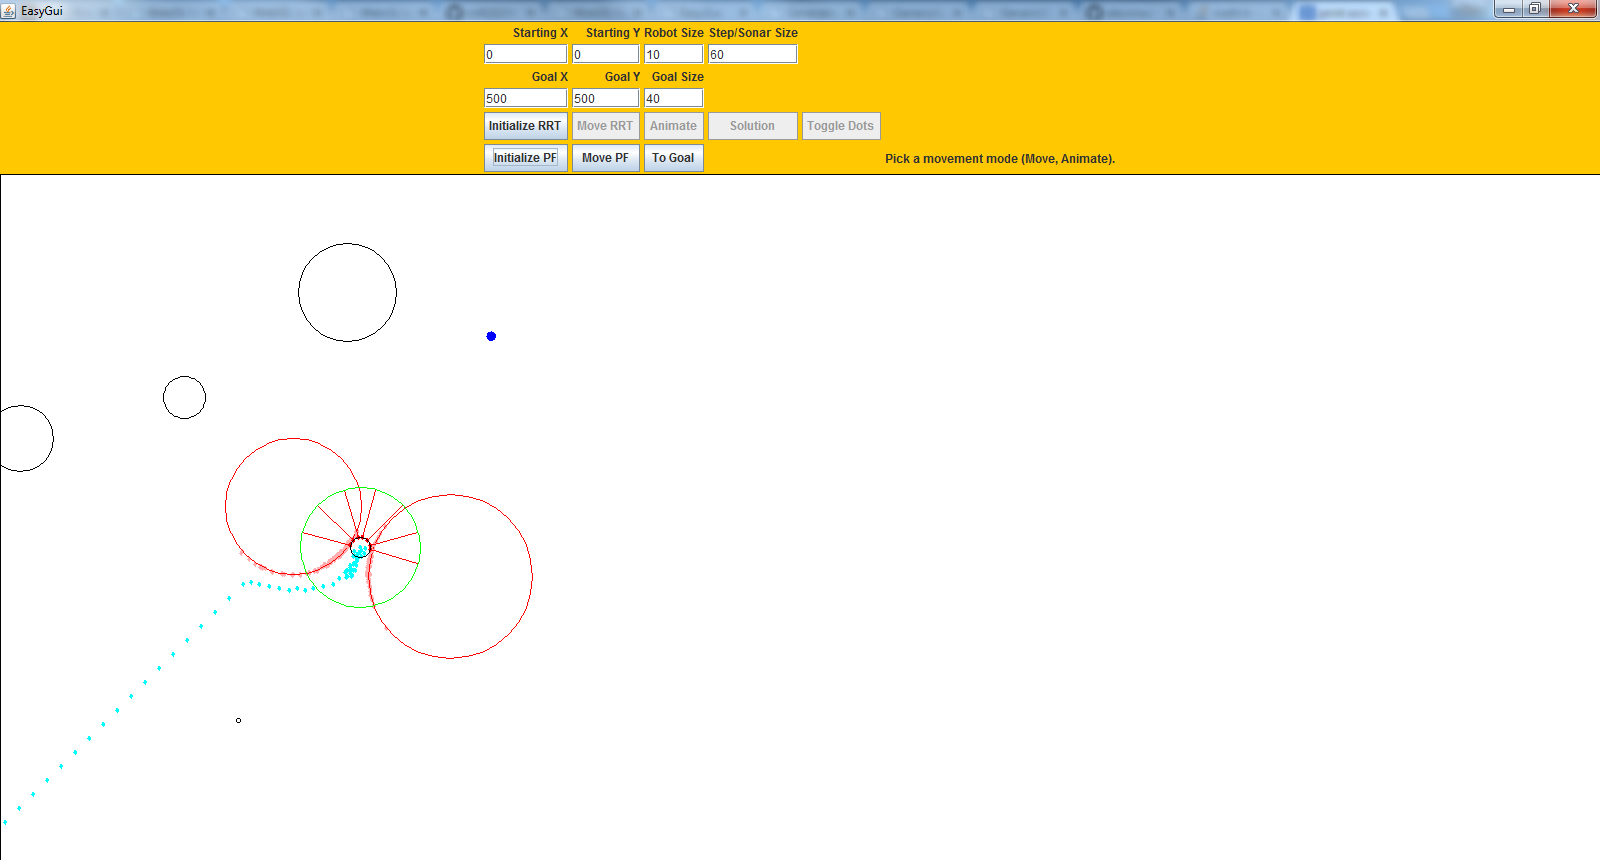
\includegraphics[width=220]{two_obstacles.png}
\caption{The PF robot stuck in a local minimum point between two obstacles.}
\end{figure}.



\end{document}

